\documentclass[12pt, a4paper, simple]{eskdtext}

\usepackage{_env/gpi_global.env}
\usepackage{_env/gpi_coursework.env}
\usepackage{_sty/gpi_u}

% Буква приложения
\def \gpiPrilLetter {А}

% Код
\ESKDletter{}{К}{Р}
\def \gpiDocTypeNum {90}
\def \gpiDocVer {00}
\def \gpiCode {\ESKDtheLetterI\ESKDtheLetterII\ESKDtheLetterIII.\gpiStudentGroupName\gpiStudentGroupNum.\gpiStudentCard-0\gpiDocNum~\gpiDocTypeNum~\gpiDocVer}

\def \gpiDocTopic {СХЕМА ПРОГРАММЫ}

% Графа 1 (наименование изделия/документа)
\ESKDcolumnI {\ESKDfontIII \gpiTopic \\ \gpiDocTopic}

% Графа 2 (обозначение документа)
\ESKDsignature {\gpiCode}

% Графа 9 (наименование или различительный индекс предприятия) задает команда
\ESKDcolumnIX {\gpiDepartment}

% Графа 11 (фамилии лиц, подписывающих документ) задают команды

% Разраб.
\ESKDcolumnXIfI {\gpiStudentSurname}

% Пров.
\ESKDcolumnXIfII {\gpiTeacherSurname}

% (пустая строка после Пров. и перед Н. контр.)
% \ESKDcolumnXIfIV {Ббббб}

% Н. контр.
\ESKDcolumnXIfV {\gpiNormalControlSurname}

% Утв.
% \ESKDcolumnXIfVI {Ввввв}

\begin{document}
\begin{ESKDtitlePage}
    \begin{flushright}
        \textbf{ПРИЛОЖЕНИЕ~\gpiPrilLetter} \enspace\enspace
    \end{flushright}
    \begin{center}
        % \gpiMinEdu \\
        \gpiEdu \\
        \gpiKaf \\
    \end{center}

    \vfill

    \begin{center}
        \gpiTopic \\
    \end{center}

    \vfill

    \begin{center}
        \textbf{\gpiDocTopic} \\
        ПО ДИСЦИПЛИНЕ \gpiDiscipline \\
    \end{center}

    \vfill

    \begin{center}
        \gpiCode \\
        Листов \pageref{LastPage} \\
    \end{center}

    \vfill

    \begin{flushright}
    \begin{minipage}[t]{.49\textwidth}
        \begin{minipage}[t]{.75\textwidth}
            \begin{flushright}
                Руководитель\\                          % Руководитель:
                \hspace{0pt}\\
                Выполнил\\                              % Выполнил
                \hspace{0pt}\\
                Консультанты:\\                         % Консультанты
                \gpiESPDInfo\\
                \gpiReviewerInfo\\
            \end{flushright}
        \end{minipage}
    \end{minipage}
    \begin{minipage}[t]{.49\textwidth}
        \begin{flushright}
            \begin{minipage}[t]{.75\textwidth}
                \gpiTeacherName~\gpiTeacherSurname\\    % Руководитель:
                \hspace{0pt}\\
                \gpiStudentName~\gpiStudentSurname\\    % Выполнил
                \hspace{0pt}\\
                \hspace{0pt}\\                          % Консультанты
                \gpiESPDName~\gpiESPDSurname\\
                \gpiReviewerName~\gpiReviewerSurname\\
            \end{minipage}
        \end{flushright}
    \end{minipage}
\end{flushright}


    \vfill

    \begin{center}
        \ESKDtheYear
    \end{center}
\end{ESKDtitlePage}


\begin{figure}[!h]
    \centering
    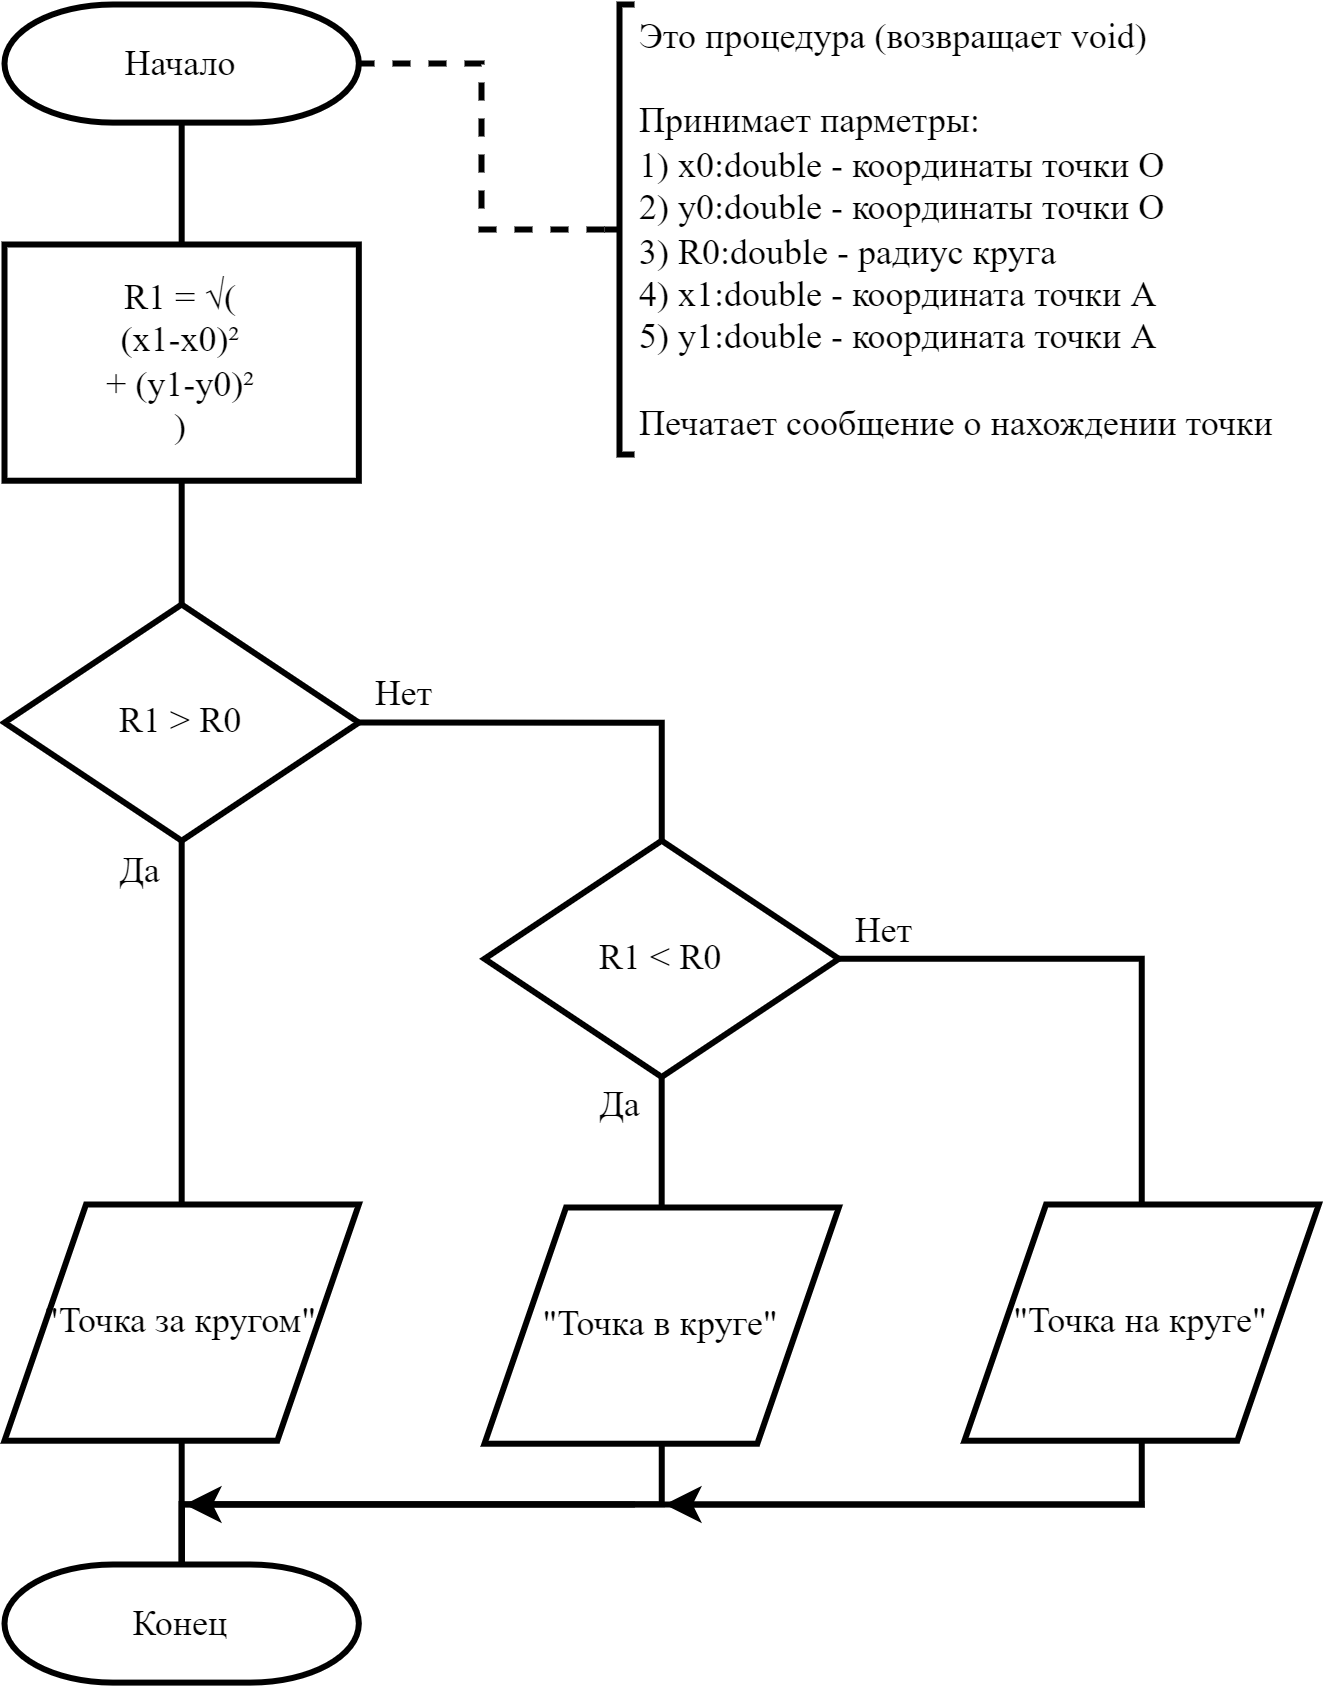
\includegraphics[]
    {../sources/flowcharts/5.png}
\end{figure}

\newpage

Вместо этого листа тут сложить горизонтальный А3 в вертикальный А4.

Как сложить смотри в видео:
\url{https://www.youtube.com/watch?v=6bhkR8yr9Rk&t=187s}

\newpage

Вместо этого листа тут сложить горизонтальный А2 в вертикальный А4.

Как сложить смотри в видео:
\url{https://www.youtube.com/watch?v=6bhkR8yr9Rk&t=140s}

\newpage

Вместо этого листа тут сложить горизонтальный А1 в вертикальный А4.

Как сложить смотри в видео:
\url{https://www.youtube.com/watch?v=6bhkR8yr9Rk}

\newpage

Вместо этого листа тут сложить горизонтальный А0 в вертикальный А4.

\newpage

Вместо этого листа тут сложить вертикальный А3 в вертикальный А4.

\newpage

Вместо этого листа тут сложить вертикальный А2 в вертикальный А4.

\newpage

Вместо этого листа тут сложить вертикальный А1 в вертикальный А4.

\newpage

Вместо этого листа тут сложить вертикальный А0 в вертикальный А4.

\newpage
\end{document}
